\card{Testing und Software-Qualitätssicherung}{
	\begin{compactenum}
		\item 3 Fault pro 1000 Zeilen Code
		\item Techniken:
		\begin{enumerate}
			
			\item Verifikations- und Validationstechniken (Codeanalyse, Bewertung, Testing, formale Verifikation), je früher desto besser (Kosten)
				\begin{enumerate}
					\item \textbf{Verifikation:} beweisen, dass ein Produkt seinen Spezifikationen entspricht (formale Verifikation (Model Checking, formale Codeverifikation (Beweise)), Korrektheitsbeweise)
					\item \textbf{Validation (Bestätigung):} experimentieren mit dem System, um zu zeigen, dass es die Anforderungen erfüllt (Simulation, Testing, Model Checking)
				\end{enumerate}
			\item Qualitätsbeurteilung des Codes (Softwaremetriken)
		\end{enumerate}
	\end{compactenum}
}

\card{SQA: Beurteilungen}{
	\begin{compactenum}
		\item technische Treffen (walk-through, Inspektionen)
		\item Ziele: SQA, Training
		\item Nicht-Ziele: Fortschrittsbewertung, Budget, Fehlerbehebung, Vergeltungsmaßnahmen (reprisals), politische Intrigen
		\item bewerten des Leiters, auf den Inhaber lautende Standards (SQA), Wartung des Orakels (Anwalt des Teufels), Schreiber, Benutzervertreter, Produzent, Kritiker
		\item auswerten vor der Bewertung
		\item bewerten des Produktes, nicht des Herstellers (Fragen stellen anstatt anzuklagen, vermeiden eines kritisierenden Stils (technische Korrektheit)
		\item Fragen aufwerfen, nicht lösen
	\end{compactenum}
}

\card{SQA: Code walk-through}{
	\begin{enumerate}
		\item "`Computer spielen"' $\Rightarrow$ "`interpretieren des Codes"'
		\item 3-5 Teilnehmer
		\item finden von Fehlern, nicht fixen
		\item Moderator, Sekretär, Prüfer, Designer (erklären des eigenen Designs)
	\end{enumerate}
}

\card{SQA: Codeinspektionen}{
	\begin{enumerate}
		\item ähnlich wie walk-through, anderes Ziel: suchen nach häufig gemachten Fehlern, keine Simulation des Verhalten des Computers
		\item nicht initialisierte Variablen, Sprünge zu/in Schleifen, nicht kompatible Zuordnungen, nicht-terminierende Schleifen, Arraygrenzen, Speicherzuweisung/-freigabe, Parametermismatch
		\item Analysetool kann hilfreich sein
	\end{enumerate}
}

\card{Testabdeckung (Coverage)}{
	\begin{enumerate}
		\item \textbf{white box testing:} Quelle ist enthüllt ((Code) strukturiertes Testing)
		\item \textbf{black box testing:} keine Quelle verfügbar (testen gegen die Anforderungsspezifikation)
		\item \textbf{grey box testing:} einige interne Zustandsvariablen sind enthüllt
	\end{enumerate}
}

\card{Testingtypen (Diagramm)}{
	\scalebox{0.95}{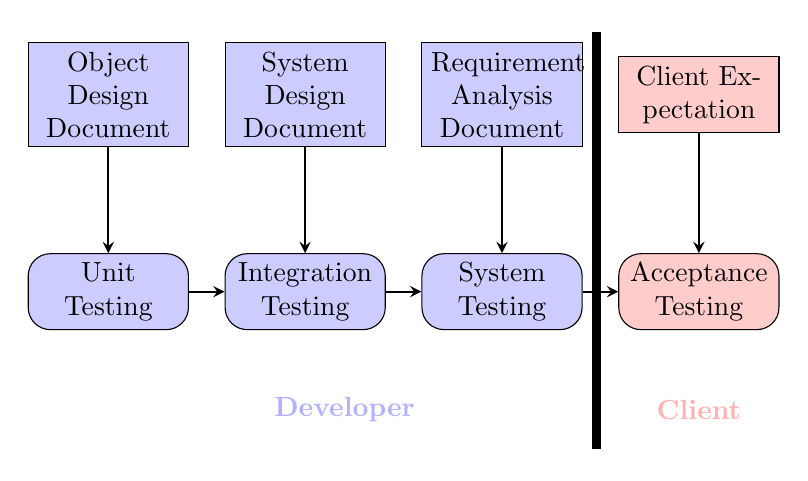
\begin{tikzpicture}[%
>=stealth,
node distance=2.5cm,
%on grid,
auto,
multiline/.style={text width=1.8cm,align=center},
square/.style={multiline,draw},
round/.style={multiline,draw,rounded corners=8pt},
dev/.style={fill=blue!20},
cl/.style={fill=red!20},
arrow/.style={draw,thick,->},
bl/.style={draw,line width=3pt}
]

\node[square,dev] (odd) at (0,0) {Object Design Document};
\node[square,dev] (sdd) [right of = odd] {System Design Document};
\node[square,dev] (rad) [right of = sdd] {Requirement Analysis Document};
\node[square,cl] (ce) [right of = rad] {Client Expectation};

\node[round,dev] (ut) [below of = odd] {Unit Testing};
\node[round,dev] (it) [below of = sdd] {Integration Testing};
\node[round,dev] (st) [below of = rad] {System Testing};
\node[round,cl] (at) [below of = ce] {Acceptance Testing};

\node (devel) at (3,-4) {\textcolor{blue!30}{\textbf{Developer}}};
\node (devel) at (7.5,-4) {\textcolor{red!30}{\textbf{Client}}};

\path[arrow] (odd) -- (ut);
\path[arrow] (sdd) -- (it);
\path[arrow] (rad) -- (st);
\path[arrow] (ce) -- (at);

\path[arrow] (ut) -- (it);
\path[arrow] (it) -- (st);
\path[arrow] (st) -- (at);

\path[bl] (6.2,.8) -- (6.2,-4.5);

\end{tikzpicture}}
}

\card{Testingtypen: Unit/Module Testing}{
	\begin{compactenum}
		\item überprüfen, ob ein Module den Designspezifikationen entspricht (oft während der Programmierung)
		\item getestet wird: Methoden im Objekt, Klassen mit mehreren Attributen/Methoden, Komponenten, die aus mehreren Klassen und internen Schnittstellen bestehen
		\item System wird nicht als Ganzes getestet
		\item gesamte Abdeckung: Testen aller Operationen mit allen möglichen Kombinationen von Parametern, sowie einstellen und testen aller möglichen Kombinationen von Objektattributwerten, sowie testen allen möglichen Zustände (Anzahl steigt schnell an)
		\item zwei Arten von Tests:
			\begin{compactenum}
				\item normal: Einheit tut, was sie tun soll
				\item Robustheitstest: wenn es einer "`feindlichen Umgebung"' ausgesetzt wird, ist die Einheit robust
			\end{compactenum}
	\end{compactenum}
}

\card{Testingtypen: Integrationstesting}{
	\begin{compactenum}
		\item wird während des Zusammenbauens des ganzen Systems ausgeführt, testet die Module zusammen, und ob das System den Anforderungen entspricht (ausgeführt mit Integratoren, getestet von Spezialisten)
		\item Driver: Komponente, die testedUnit aufruft, Testfälle kontrolliert
		\item Stub: Komponente, von der die testedUnit abhängt ("`Fake"')
		\item Testmethoden:
			\begin{compactenum}
				\item \textbf{big bang:} zusammenfügen und sehen, ob es funktioniert
				\item \textbf{top-down:} testen die oberste Schicht zuerst, dann abwärts (Stubs sind notwendig, Test kann durch die Funktionalität des Systems entworfen werden)
				\item \textbf{bottom-up:} Untersysteme in der untersten Schicht werden zu erst getestet (Drivers sind notwendig (Testen des UI (wichtigster Teil) zum Schluss)
				\item \textbf{sandwich:} Kombination von bottom-up und top-down, konvergiert auf der Zielebene
				\item \textbf{modified sandwich:} Kombi aller anderen Testmethoden
			\end{compactenum}
	\end{compactenum}
}

\card{Testingtypen: Systemtesting}{
	testen des System als Ganzes
}

\card{Testingtypen: Akzeptanztesting}{
	\begin{enumerate}
		\item testet, wie der Kunde benutzt, wenn sie geliefert wurde (kann behoben werden in der Anforderungsspezifikation oder im Vertrag)
		\item demonstriert, dass das System bereit für den betrieblichen Einsatz ist
		\item Auswahl von Tests von Kunden, durchgeführt vom Kunden
		\item kann Teil des Vertrages sein
		\item Alpha Tests: Tests in Entwicklungsumgebung\\
		Beta Tests: Tests in Kundenumgebung
	\end{enumerate}
}

\card{Testingtypen: Regressionstesting}{
	ausgeführt während der Wartung/ wenn sich eine Komponente verändert hat (sicherstellen, dass das was vorher funktioniert hat auch weiterhin funktioniert)
}

\card{Testingtypen: Stresstesting}{
	testen des Systems unter extremen Bedingungen
}

\card{Testing: Dijkstra}{
	"`Programmtesting kan benutzt werden um zu zeigen, dass ein Fehler vorliegt, aber niemals um zu zeigen, dass es keinen Fehler gibt."'\\
	Man muss immer genau schauen, welchen Teil des Systems man mit seinem Testing erreicht (Test-Coverage).
}

\card{formelles Testing}{
	\begin{compactitem}[\leftmargin=0pt]
		\item[\textbf{D:}] Eingabe Domain, \textbf{R:}  beliebige Menge, Ergebnis
		\item[\textbf{P:}] Teilfunktion, beschreibt das Verhalten des Programms bei Input/Output:\\
				$P: D \rightarrow R$
		\item[\textbf{OR:}] Ausgabewert der Anforderungen (aus dem SRS)
	\end{compactitem}
	\textbf{testing:} bestimmen ob für ein gegebenes $d \in D, P(d) $ die Anforderungen erfüllt sind (angegeben in OR), falls ja $\Rightarrow$ Erfolg, ansonsten \textit{fail}
	\begin{compactitem}[\leftmargin=0pt]
		\item[$d \in D$:] Testfall (Test Case)
		\item[$T \subseteq D$:] Testmenge/-folge
		\item[T:] ist erfolgreich, gdw. alle $d \in T$ erfolgreich sind
		\item[$C \subseteq 2_f^D$:] Auswahlkriterium, $2_f^D$ ist Menge aller endl. Teilmengen von D
		\item[T:] erfüllt C gdw. $T \in C$
		\item[für alle $i,k$:] nehmen an, dass $T_i, T_k$ erfüllt C, C ist konsistent, falls ($T_i$ ist erfolgreich, gdw. $T_k$ ist erfolgreich)
		\item[C:] ist komplett, falls P nicht korrekt, so gibt es T(nicht erfolgreich) das C erfüllt
	\end{compactitem}
	falls C komplett und konsistent: jeder Test T erfüllt C entscheidet P's Korrektheit
}

\card{Selektives Testing - wie viele Pfade muss man testen? (Coverage)}{
	\begin{description}
		\item[Statement Coverage:] Jedes Statement wird mindestens einmal besucht
		\item[Edge Coverage:] Jede Kante wird genau einmal traversiert
		\item[Condition Coverage:] Edge Coverage ist erfüllt und alle möglichen Werte für die Bestandteile der Aussage innerhalb der \textit{Conditions} wird mindestens einmal ausgeführt
		\item[Multiple Condition Coverage:]  Jede boolesche Kombination der Bedingungen in jeder \textit{Condition} muss mindestens einmal ausgeführt werden
		\item[Path Coverage:] Alle Pfade von einem Startknoten zu einem Endknoten müssen mindestens einmal durchlaufen werden
	\end{description}
}

\card{Basic Path Testing}{
	\begin{enumerate}
		\item beurteilen wie viele Tests benötigt sind, um Aussagen und Path Coverage zu erreichen (Programm ist ein einzelner Eintrag, einfacher Ausgang, Kontrollflussgraph verfügbar, alle Entscheidungen sind Binär)
		\item berechnen der \textit{cyclomatic complexity V(G)}: $V(G) = \# $ einfacher Entscheidungen + 1 = $\#$ abgeschlossener Flächen + 1
		\item Schleifentesten (n ist Anzahl erlaubter Durchläufe)
			\begin{compactenum}
				\item überspringen der Schleife
				\item erster Durchlauf
				\item zweiter Durchlauf
				\item m Durchläufe ($m < n$)
				\item $(n-1),n,(n+1)$ Durchläufe
			\end{compactenum}
	\end{enumerate}
}

\card{Testen auf Grundlage von Verträgen (mögliche Testauswahlkriterien)}{
	\begin{enumerate}
		\item Input entspricht der Precondition
		\item Inputs mit verletzter Precondition
		\item Inputs, bei dem das Key-Element den richtigen Typ hat
		\item Inputs, bei dem das Key-Element den falschen Typ hat
	\end{enumerate}
}

\card{Testplan}{
	\begin{enumerate}
		\item Systemübersicht
		\item Features zum Testen und Nicht-Testen (funktionale Aspekte, Beschreibung der zu testenden Features)
		\item Kriterien für "`Fail"' oder "`Pass"'
		\item Herangehensweise an Testprozess, Begründung zur Wahl der Testmethode
		\item Testfälle
			\begin{compactenum}
				\item Testfallbezeichner
				\item Testitems
				\item Eingabe- und Ausgabespezifikation
				\item Umgebungsanforderungen (Hardware, Software)
				\item besondere prozedurale Anforderungen (Zeitlimits, \dots)
				\item Abhängigkeiten zwischen Testfällen
			\end{compactenum}
	\end{enumerate}
}

\card{Äquivalenzklassenbildung}{
	Aufsplitten der Inputdomain in zwei äquivalente Klassen, sodass jede Eingabeklasse so viele Programmfehler wie möglich aufzeigt. Zur Bestimmung der Äquivalenzklassen: schauen auf die Eingabebedingungen des Systems.\\
	Testen \textbf{eines Wertes} für jede Äquivalenzklasse.
}